
% preamble to the OGTC logic report compiler
% This piece of code consists of initializing
% the code and declaring colors, packages and 
% command changes such as the section headings
% the document is aimed to be as consise as possible
% please keep this in mind when expanding or 
% editing the code


\documentclass{article}[11pt]
%% declare used packages
\usepackage{lipsum}
\usepackage[english]{babel}
\usepackage[defaultfam,tabular,lining]{montserrat} 
\usepackage{geometry}
 \geometry{a4paper, total={170mm,257mm}, left=15mm, right = 15mm, top=40mm, bottom =30mm}
\usepackage{multicol} % multiple columns
\usepackage{fancyhdr} % header and footer
\usepackage{titlesec} % remove spacing around section titles, underline section titles
\usepackage{tikz}     % header and footer
\usepackage{currency} % euro sign
\usepackage{caption}
\usepackage{setspace}
%\usepackage{amsmath}
%% Declares the logic blue

\definecolor{primblue}{RGB}{2,81,151} %giuls code
%\definecolor{primblue}{RGB}{40,53,131} %Mariens laptop
%% Declare main text color
\definecolor{maintext}{RGB}{59, 56, 56}
\color{maintext}
% define euro as currency
\DefineCurrency{EUR}{name={euro},pre=true,plural={euros},symbol={\euro},iso={EUR},kind=symbol,base=2}

% page style
\usetikzlibrary{calc}
\renewcommand{\headrulewidth}{0pt}

\pagestyle{fancy}
\fancyhf{}
\fancyhead[C]{%
\begin{tikzpicture}[overlay, remember picture]%
    \fill[primblue] (current page.north west) rectangle ($(current page.north east)+(0,-1in)$);
    \node[anchor=north west, text=white, font=\LARGE\scshape, minimum size=1in, inner xsep=15mm,text width = 12cm] at (current page.north west) {\textbf{Your microgrid assessment by OGTC} \large Powered by LOGiC};
    \node[anchor=north east, minimum size=1in, inner xsep=5mm] at (current page.north east) {
\includegraphics[scale=.1]{logo.png}};
      %node[minimum width=\x2-\x1, minimum height=2cm, draw, rectangle, fill=blue!20, anchor=north west, align=left, text width=\x2-\x1] at ($(current page.north west)$) {\Large\bfseries \quad #1};
\end{tikzpicture}
}

\fancyfoot[CO]{
    \begin{tikzpicture}[overlay, remember picture]%
    \fill[primblue] (current page.south west) rectangle ($(current page.south east)+(0,.5in)$);
    \node[anchor=south west, text=white, font=\large, minimum size=.5in, inner xsep=5mm] at (current page.south west) {www.offgridtestcenter.nl};
    \node[anchor=south, text=white,  font=\large, minimum size=.5in] at (current page.south) {\leftmark};
    \node[anchor=south east, text=white, font=\large, minimum size=.5in, inner xsep = 5mm] at (current page.south east) {info@offgridtestcenter.nl};
\end{tikzpicture}
}
%\setlength{\headheight}{12pt}
\setlength\columnsep{10mm}
\renewcommand{\arraystretch}{0.8} % makes line spacing in tables bigger
\titlespacing*{\section}{0pt}{2.5mm}{0mm} % make spacing smaller

\titleformat{\section}
    {\vspace{20pt}\color{primblue}\titlerule[6pt]\normalfont\LARGE\bfseries\color{primblue}}{\thesection}{1em}{}[\color{primblue}\titlerule\vspace*{4pt}]
\let\oldtitleline\titleline


\titleformat{\subsection}
    {\normalfont\Large\bfseries\color{primblue}}{\thesection}{1em}{}[\color{primblue}\titlerule\vspace*{4pt}]
\let\oldtitleline\titleline
\renewcommand{\titleline}{\oldtitleline*}
\setlength{\titlewidth}{0.25\textwidth}
    
\newenvironment{Figure}
  {\par\medskip\noindent\minipage{\linewidth}}
  {\endminipage\par\medskip}

\renewcommand{\baselinestretch}{1.5}

\DeclareCaptionFont{lab}{\color{black}}
\DeclareCaptionFont{txt}{\color{black}}
%% set up captions
\captionsetup[figure]{labelfont = {lab,it,footnotesize},textfont = {txt,it,footnotesize}, justification=raggedright, singlelinecheck = false} % or: footnotesize
\captionsetup[table]{labelfont = {lab,it,footnotesize},textfont = {txt,it,footnotesize}, justification=raggedright, singlelinecheck=false} % or: footnotesize

\begin{document}

\begin{large} \noindent {\setstretch{1.0}\color{primblue} This document shortly reports the results of the use of the OGTC Microgrid Assessment Tool. The tool has been used to assess a possible microgrid located at or close to dumadr.} \end{large}

\section*{Microgrids}\begin{multicols}{2}\setlength{\parindent}{0pt}

In order to make this report comprehendable to the user the general properties of a microgrid are shortly discussed.\\ A microgrid is a local energy system that is capable of generating, storing and delivering energy locally. Microgrids can be both connected to the main grid (grid-connected microgrids) as well as being completely isolated (off-grid microgrids). The microgrid considered in this assessment is a off-grid microgrid. This means that the microgrid has to generate all electrical energy consumed in the grid locally and that no extra energy can be bought from external parties. Shortages are fulfilled by using a back-up diesel generator. There are multiple possible reasons to apply a microgrid: \begin{itemize}

 \item No grid is available (remote location) 

\item There is a grid availble, but is is not reliable (enough)  

\item The wish to generate the own energy locally as a stakeholder or a community 

\end{itemize}

In all cases renewable sources are often considered as a possible source of energy for the microgrid, either from an economic or a sustainable drive. In the case of this microgrid the following sources are considered: wind power, solar power and a back-up generator combined with a storage facility.

\end{multicols}\section*{Your microgrid}\begin{multicols}{2}\setlength{\parindent}{0pt}

The assessed situation results in the mircogrid configuration and associated economics described below.

\subsection*{System sizing}

The calculation described above has resulted in the following system:

{\color{black}\begin{flushleft}

\begin{tabular}{|l|r|r|}

\hline Component&Capacity&Unit\\ \hline 

Installed solar power&184.63&kWp\\ 

Installed wind power&151.59&kW\\ 

Installed backup power&33.25&kW\\ 

Installed storage capacity&478.38&kWh\\ 

Power of storage facility&239.19&kW\\ 

\hline

\end{tabular}

\label{tab:systemlayout}

\end{flushleft}}\captionof{table}{Sizing of the main components of the system}\vspace{0.5mm}

The system defined by the parameters above realises a levelised cost of electricity of \texteuro 0.31 per kWh. the system does this at a renewable energy share of 90.3 \%. 

\subsection*{System economics}

In order to assess the economics of the system the following economic parameters have been assumed: 

{\color{black}\begin{flushleft}

\begin{tabular}{|l|r|r|}

\hline Variable&Value&Units\\ \hline 

Fuel price&1.22&\euro /liter\\ 

Annual change in fuel price&0.05&\euro /liter\\ 

Import tax&21.00&\%\\ 

WACC&2.00&\%\\ 

\hline

\end{tabular}

\label{tab:econinputtable}

\end{flushleft}}\captionof{table}{Economic input variables}\vspace{0.5mm}

The investment costs associated with the use of the different main components are assumed to be:

{\color{black}\begin{flushleft}\begin{tabular}{|l|r|r|}\hline Component&Investment costs&Units\\ \hline 

Solar&\texteuro \hfill2,800.00&kWp\\ 

Wind&\texteuro \hfill2,500.00&kW\\ 

Backup generator&\texteuro \hfill820.00&kW\\ 

Storage capacity&\texteuro \hfill20.00&kWh\\ 

Storage power&\texteuro \hfill500.00&kW\\ 

\hline

\end{tabular}

\label{tab:investinputtable}

\end{flushleft}}\captionof{table}{Per unit investment cost of the main considered system components}\vspace{0.5mm}

Based on these the investment costs of the main components of the system are estimated as:

{\color{black}\begin{flushleft}\begin{tabular}{|l|r|}\hline Component&Investment cost\\ \hline 

Solar modules&\texteuro \hfill575,884.65\\ 

Wind turbines&\texteuro \hfill458,572.91\\ 

Backup generator&\texteuro \hfill60,076.57\\ 

Storage facility&\texteuro \hfill266,683.58\\ 

\hline

\end{tabular}

\label{tab:investtable}

\end{flushleft}}\captionof{table}{Investment cost of the system}\vspace{0.5mm}

The operational expenditure is estimated as:

{\color{black}\begin{flushleft}\begin{tabular}{|l|r|r|}\hline Component&Annual pu OPEX&Units\\ \hline 

Solar panels&\texteuro \hfill25.00&kWp\\ 

Wind turbines&\texteuro \hfill0.00&kW\\ 

Backup generator&\texteuro \hfill0.05&kW\\ 

Storage capacity&\texteuro \hfill6.75&kWh\\ 

Storage power&\texteuro \hfill0.00&kW\\ 

\hline

\end{tabular}

\label{tab:opextable}

\end{flushleft}}\captionof{table}{Operational expenditure of the main components of the system}\vspace{0.5mm}



\end{multicols}\section*{Method}\begin{multicols}{2}\setlength{\parindent}{0pt}

The OGTC Microgrid Assessment Tool utilizes the Open Energy MOdelling Framework (OEMOF) to make a first estimation of the (economical) optimal size of the generation and storage components in an (off-grid) microgrid. This estimation is made by deriving an equation that describes the cost of energy of a microgrid with the chosen components and solving for the lowest system cost. 

The total electricity demand has been been specified as 365250 kWh per year and has been converted to a demand time series using historic load data collected by ENTSO-E.

The expected energy production by solar panels and wind turbines has been estimated based on weather data made available by the PVGIS project. This weather data (solar radiation and windspeed) has been used to calculate the expected generated power per installed kW of wind power and kWp of solar power, respectively. \vfill\null\columnbreak\appendix

\subsection*{Used input data and method}

The timeseries used in and resulting from the calculations are listed on this page.

\begin{center}

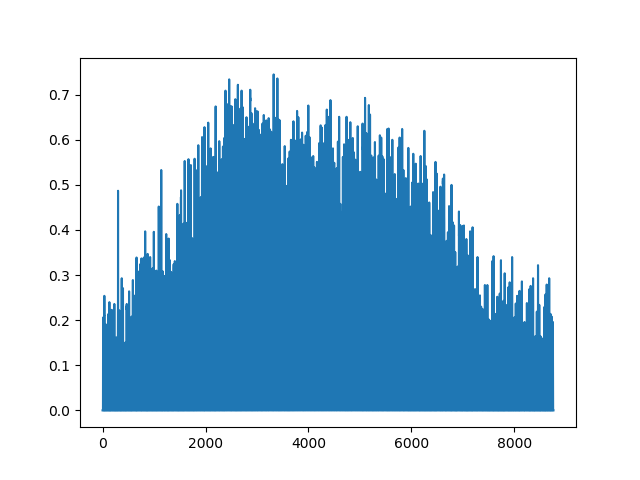
\includegraphics[width=\linewidth]{per_unit_pv_generation.png}

\end{center}

\captionof{figure}{Time series of the solar energy production in kW per kWp of installed solar power}





\begin{center}

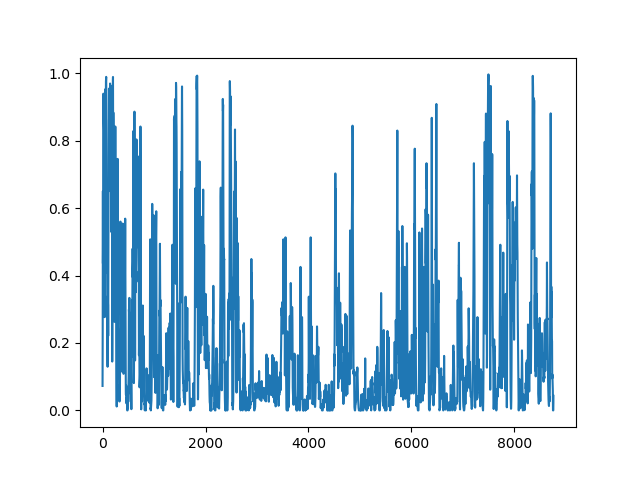
\includegraphics[width=\linewidth]{per_unit_wind_generation.png}

\end{center}

\captionof{figure}{Time series of the wind energy production in kW per kW of installed wind power}







\end{multicols}\section*{Contributors}\begin{multicols}{2}\setlength{\parindent}{0pt}

The Microgrid Assessment Tool has been developed by the LOGiC Team at the Off Grid Test Center. 

The tool is based on the Offgridders tool, initially developed by Martha Hoffmann at the Reinier Lemoin Instute in Berlin, Germany. 

Based on this work and with financial support by LOGiC the team was able to succesfully developt this implementation. 

Other contributers to the tool are: 

\begin{itemize}

\item Alex and Stan Bankras at Stalex (web development)

\item Ewout van der Beek at NEDU (data interpretation)

\item Wind Energy Solutions BV (general support)

\end{itemize}

\vfill

\begin{center}


\includegraphics[width=\linewidth]{logiclogo.png}

\end{center}

\centering \small{The OGTC MAT is powered by LOGiC}

\end{multicols}

\end{document}